\documentclass[a4paper]{article}
\usepackage[margin = 0.8in]{geometry}
\setlength{\parskip}{0.7\baselineskip}
\linespread{1.4}
\usepackage[]{graphicx}
\usepackage{amsmath}
\usepackage{amssymb}
\usepackage{float}
\usepackage{braket}
\usepackage{siunitx}
 \usepackage{verbatim}
%\usepackage{physics}
%\usepackage{tikz-feynman}
%\usepackage{slashed}
%\usepackage{simpler-wick}
\usepackage{xcolor}
%\usepackage[style=footnote-dw]{biblatex}
\newcommand{\normord}[1]{:\mathrel{#1}:}
% Package biblatex: '\bibliography' must be given in preamble.
\begin{document}

\begin{figure}[H]
  \centering
  \includegraphics[width=0.23\textwidth]{v1-g1_abs.png}
  \includegraphics[width=0.23\textwidth]{v1-g2_abs.png}
  \includegraphics[width=0.23\textwidth]{v1-g3_abs.png}
  \includegraphics[width=0.23\textwidth]{v1-g4_abs.png}
  \includegraphics[width=0.23\textwidth]{v2-g1_abs.png}
  \includegraphics[width=0.23\textwidth]{v2-g2_abs.png}
  \includegraphics[width=0.23\textwidth]{v2-g3_abs.png}
  \includegraphics[width=0.23\textwidth]{v2-g4_abs.png}
  \includegraphics[width=0.23\textwidth]{v3-g1_abs.png}
  \includegraphics[width=0.23\textwidth]{v3-g2_abs.png}
  \includegraphics[width=0.23\textwidth]{v3-g3_abs.png}
  \includegraphics[width=0.23\textwidth]{v3-g4_abs.png}
\end{figure}

\begin{figure}[H]
  \centering
  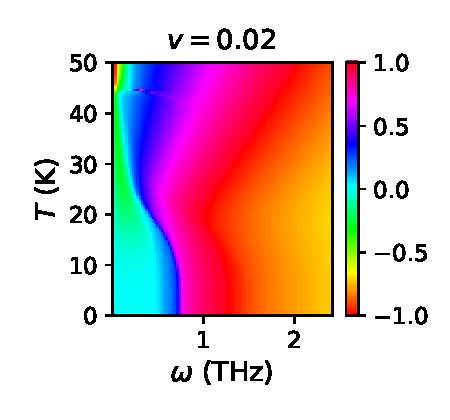
\includegraphics[width=0.23\textwidth]{v1-g1_phase.png}
  \includegraphics[width=0.23\textwidth]{v1-g2_phase.png}
  \includegraphics[width=0.23\textwidth]{v1-g3_phase.png}
  \includegraphics[width=0.23\textwidth]{v1-g4_phase.png}
  \includegraphics[width=0.23\textwidth]{v2-g1_phase.png}
  \includegraphics[width=0.23\textwidth]{v2-g2_phase.png}
  \includegraphics[width=0.23\textwidth]{v2-g3_phase.png}
  \includegraphics[width=0.23\textwidth]{v2-g4_phase.png}
  \includegraphics[width=0.23\textwidth]{v3-g1_phase.png}
  \includegraphics[width=0.23\textwidth]{v3-g2_phase.png}
  \includegraphics[width=0.23\textwidth]{v3-g3_phase.png}
  \includegraphics[width=0.23\textwidth]{v3-g4_phase.png}
\end{figure}

\end{document}
 
 
